\documentclass[a4paper]{article}

\usepackage{array}
\usepackage{listings}
\usepackage{appendix}
\usepackage{hyperref}
\usepackage{graphicx}
\usepackage{numprint}
\usepackage{booktabs}
\usepackage{subcaption}
\usepackage{listings}
\usepackage[T1]{fontenc}

\usepackage{hyperref}
\hypersetup{
  colorlinks=true,
  linkcolor=blue,
  filecolor=magenta,
  urlcolor=cyan,
}
\npdecimalsign{.}
\nprounddigits{4}

\title{Raijin to Gadi Transition Consistency Tests for Processing Landsat Collection 3}
\date{16 March 2020}
\author{Analysis Read Data\\ Pipelines and Data Workflows Team}

\begin{document}
  \pagenumbering{gobble}
  \maketitle
  \newpage
  \pagenumbering{arabic}

  \section{Introduction}

    \begin{flushleft}
      The National Computational Infrastructure (NCI) Australia is shutting down the Raijin compute cluster and moving to the Gadi compute cluster. This can have an impact on the consistency on data products, with the worst case scenario being the archive needs to be reprocessed. \par
      This report aims to present information regarding the consistency of the output products when using a different processing environment to output Digital Earth Australia's Landsat Collection 3 products.. \par
      The report is not a reflection of the Gadi compute cluster, nor a suggestion that there is anything wrong with the Gadi compute cluster. \par
      Reports on the analytical findings regarding the consistency of any Collection level processing should be undertaken when setting up any new processing pipelines.
    \end{flushleft}

    \subsection{Processing environments}
    \label{sec:environ}
      \begin{itemize}
        \item Raijin
          \begin{itemize}
            \item wagl-5.4.0 (Compiled with GCC-5.2.0)
            \item eugl-0.2.0
            \item tesp-0.6.1
            \item eodatasets3-0.6.0
            \item fmask-0.5.4
            \item gverify-0.25v
            \item MODTRAN-6.0.1
          \end{itemize}
        \item Gadi
          \begin{itemize}
            \item wagl-5.4.1 (Compiled with GCC-8.2.1)
            \item eugl-0.2.1
            \item tesp-0.6.2
            \item eodatasets3-0.6.0
            \item fmask-0.5.4
            \item gverify-0.25v
            \item MODTRAN-6.0.1
          \end{itemize}
      \end{itemize}

    \subsection{Base input data}

      USGS Landsat Collection-1 Level-1 Landsat-8

    \subsection{Acquisition Period}

      2019-05

    \subsection{Reported Metrics}
      \begin{itemize}
        \item Minimum residual
        \item Maximum residual
        \item Percentage of pixels that are different
        \item Min and Max percentage of pixels that have changed categorical value
      \end{itemize}

    \subsection{Measurements}
      \begin{itemize}
        \item nbar\_coastal\_aerosol
        \item nbart\_coastal\_aerosol
        \item nbar\_blue
        \item nbart\_blue
        \item nbar\_green
        \item nbart\_green
        \item nbar\_red
        \item nbart\_red
        \item nbar\_nir
        \item nbart\_nir
        \item nbar\_swir\_1
        \item nbart\_swir\_1
        \item nbar\_swir\_2
        \item nbart\_swir\_2
        \item nbar\_panchromatic
        \item nbart\_panchromatic
        \item oa\_fmask
        \item oa\_combined\_terrain\_shadow
        \item oa\_nbar\_contiguity
        \item oa\_nbart\_contiguity
        \item oa\_solar\_azimuth
        \item oa\_solar\_zenith
        \item oa\_satellite\_azimuth
        \item oa\_satellite\_view
        \item oa\_azimiuthal\_exiting
        \item oa\_azimiuthal\_incident
        \item oa\_exiting\_angle
        \item oa\_incident\_angle
      \end{itemize}

    \subsection{Other Assessments}
      \begin{itemize}
        \item GQA (Geometric Quality Assessment)
        \item Software Versions
        \item File Naming Consistency
        \item Quicklook Images
      \end{itemize}

    \section{Method}

      \begin{flushleft}
        Landsat-8 Level-1 acquisitions for the month of May 2019 (approx 1000 granules) and processed on the Raijin compute cluster were used as input in the test production environment built on the Gadi compute cluster. \par
        The output product \textit{ga\_ls8c\_ard\_3} processed on the Gadi compute cluster was then compared with the \textit{ga\_ls8c\_ard\_3} product processed on the Raijin compute cluster.
      \end{flushleft}

    \subsection{Rationale}

      \begin{flushleft}
        Depending on the software versions being compared, it is expected that there will be change and the idea is to build a general understanding of the type of change that is occurring, be that large or small; not to define the explicit details of why a change has occurred. \par
        While extrema are reported (maximal and minimal residuals), they are often misinterpreted leading to biased assumptions as they don't describe the proportionality of change. The proportionality of change is what the aforementioned metrics are designed to describe. \par
        Initially, the metrics were designed to inform the operations team of a potential change in the underlying data, thus requiring further investigation and potentially leading to a recommendation to the leadership team for a collection upgrade. \par
        The percent different was simply describing the proportionality of change. For routine integration tests, it is ideal to have this number closer 0. As routine testing that is occurring on the same machine should exhibit less noise in floating point calculations. If deploying the codebase to a different machine, it is expected that there will be some floating point differences. This can occur due to slight differences in machine architecture, and/or different compilers. As such, this metric coupled with minimal and maximal differences/residuals, can help in aiding a user to ignore noise such as compiler or machine architecture differences. \par
      \end{flushleft}

  \newpage

  \section{Results}

    \subsection{Continental overview}

    \begin{flushleft}
      The following tables are reporting on the extrema (min and max) of difference for the different processing environments. \par
      The results for every acquisition within the month of May 2019 are aggregated into their respective spatial regions and evaluated to find the total minimum and maximum of change in percent reflectance for a given measurement across the continent. \par
    \end{flushleft}

    \begin{table}[ht!]
      \caption{Minimum difference in surface reflectance (units are \% reflectance)}\label{table:1}
      \centering
      \begin{tabular}{cc} \midrule
        \textbf{Measurement} & \textbf{Minimum} \\ \midrule
        nbar\_coastal\_aerosol & -0.33 \\
        nbart\_coastal\_aerosol & -0.33 \\
        nbar\_blue & -0.24 \\
        nbart\_blue & -0.24 \\
        nbar\_green & -0.12 \\
        nbart\_green & -0.12 \\
        nbar\_red & -0.07 \\
        nbart\_red & -0.07 \\
        nbar\_nir & -0.03 \\
        nbart\_nir & -0.05 \\
        nbar\_swir\_1 & -0.06 \\
        nbart\_swir\_1 & -0.06 \\
        nbar\_swir\_2 & -0.07 \\
        nbart\_swir\_2 & -0.08 \\
        nbar\_panchromatic & -0.12 \\
        nbart\_panchromatic & -0.13 \\ \midrule
      \end{tabular}
    \end{table}

    \begin{table}[ht!]
      \caption{Maximum difference in surface reflectance (units are \% reflectance)}\label{table:2}
      \centering
      \begin{tabular}{cc} \midrule
        \textbf{Measurement} & \textbf{Maximum} \\ \midrule
        nbar\_coastal\_aerosol & 0.26 \\
        nbart\_coastal\_aerosol & 0.28 \\
        nbar\_blue & 0.18 \\
        nbart\_blue & 0.19 \\
        nbar\_green & 0.13 \\
        nbart\_green & 0.12 \\
        nbar\_red & 0.13 \\
        nbart\_red & 0.13 \\
        nbar\_nir & 0.11 \\
        nbart\_nir & 0.11 \\
        nbar\_swir\_1 & 0.11 \\
        nbart\_swir\_1 & 0.11 \\
        nbar\_swir\_2 & 0.1 \\
        nbart\_swir\_2 & 0.1 \\
        nbar\_panchromatic & 0.11 \\
        nbart\_panchromatic & 0.11 \\ \midrule
      \end{tabular}
    \end{table}

  \newpage

    \begin{table}[ht!]
      \caption{Maximum difference for the angular measurements (units are degrees)}\label{table:3}
      \centering
      \begin{tabular}{cc} \midrule
        \textbf{Measurement} & \textbf{Maximum} \\ \midrule
        oa\_solar\_azimuth & 0.0 \\
        oa\_solar\_zenith & 0.0 \\
        oa\_satellite\_azimuth & 282.2354736328125 \\
        oa\_satellite\_view & 11.190152168273926 \\
        oa\_azimuthal\_exiting & 362.8235168457031 \\
        oa\_azimuthal\_incident & 362.8235168457031 \\
        oa\_exiting\_angle & 3.0386683391725455e-08 \\
        oa\_incident\_angle & 0.0026793109718710184 \\ \midrule
      \end{tabular}
    \end{table}

    \begin{flushleft}
      Table~\ref{table:4}, below, represents the proportion of pixels that a different (excluding those pixels that may have changed to a \textit{Null} or vice versa). The maximum percent different for each measurement is derived from a continental aggregation.
    \end{flushleft}

    \begin{table}[ht!]
      \caption{Percentage of pixels (acquisition wide) that are different}\label{table:4}
      \centering
      \begin{tabular}{cc} \midrule
        \textbf{Measurement} & \textbf{Percentage} \\ \midrule
        nbar\_coastal\_aerosol & 0.09190939962673991 \\
        nbart\_coastal\_aerosol & 0.09248046758124409 \\
        nbar\_blue & 0.0936635450166426 \\
        nbart\_blue & 0.0945747004380302 \\
        nbar\_green & 0.08982254804615988 \\
        nbart\_green & 0.09079931432535389 \\
        nbar\_red & 0.1013562413386793 \\
        nbart\_red & 0.10051996510454053 \\
        nbar\_nir & 0.05485456466504311 \\
        nbart\_nir & 0.06778161124419617 \\
        nbar\_swir\_1 & 0.04232365890372 \\
        nbart\_swir\_1 & 0.05250500364041894 \\
        nbar\_swir\_2 & 0.049452682100564825 \\
        nbart\_swir\_2 & 0.05921647001836844 \\
        nbar\_panchromatic & 0.07109107169514148 \\
        nbart\_panchromatic & 0.08812408383484639 \\
        oa\_solar\_azimuth & 0.0 \\
        oa\_solar\_zenith & 0.0 \\
        oa\_satellite\_azimuth & 0.1524497668024873 \\
        oa\_satellite\_view & 11.190152168273926 \\
        oa\_azimuthal\_exiting & 11.21063871988424 \\
        oa\_azimuthal\_incident & 9.361480335090448 \\
        oa\_exiting\_angle & 37.16646032657571 \\
        oa\_incident\_angle & 30.180973333954185 \\ \midrule
      \end{tabular}
    \end{table}

      \begin{flushleft}
        The minimum and maximum difference are all reporting less than 1\% change in surface reflectance. \par
        This is unlikely to have a significant impact on DEA's products derived from this baseline. Aquatic remote sensing applications, such as suspended sediment concentration, may find this significant, however, it is recommended not to be using be using DEA's NBAR or NBART surface reflectance product for such applications. \par
        Applications identifying surface water may be less impacted than those measuring content within water bodies. \par
        The maximum proportion of differences for the surface reflectance bands is also less than 1\%, indicating minimal change from all acquisition over the continent for the month of May 2019. \par
        For datasets containing angular measurements, there are large distribution of pixels that are different. However, as the minimal and maximal differences are quite small and have had little impact on the output surface reflectance, it is most likely due to differences in floating point calculations.
      \end{flushleft}

      \begin{flushleft}
        Table~\ref{table:5} and Table~\ref{table:6}, below, represents the minimum and maximum percentage of pixels in a given category within the Fmask schema changing to another category. i.e. Pixels originally classified as Clear and now being classified as Cloud. \par
        A value of 100 represents 100\%, and indicates that all pixels from all granules mapped entirely to the corresponding category. A NaN implies no recorded pixels for that category. \par
        A good indicator for data consistency for a category mapping to the same category, say cloud to cloud, is a value close to 100\%. For a category mapping to a different category, say cloud to snow, a value close to 0\% or NaN, is also good indicator for data consistency.
      \end{flushleft}

  \clearpage

    \begin{table}[ht!]
      \caption{Minimum percentage of categorical change within Fmask}\label{table:5}
      \centering
      \begin{tabular}{ccccccc} \midrule
        & \textbf{Null} & \textbf{Clear} & \textbf{Cloud} & \textbf{Cloud Shadow} & \textbf{Snow} & \textbf{Water} \\ \midrule
        \textbf{Null} & 100 & NaN & NaN & NaN & NaN & NaN \\
        \textbf{Clear} & NaN & 100 & NaN & NaN & NaN & NaN \\
        \textbf{Cloud} & NaN & NaN & 100 & NaN & NaN & NaN \\
        \textbf{Cloud Shadow} & NaN & NaN & NaN & 100 & NaN & NaN \\
        \textbf{Snow} & NaN & NaN & NaN & NaN & 100 & NaN \\
        \textbf{Water} & NaN & NaN & NaN & NaN & NaN & 100 \\
      \end{tabular}
    \end{table}

    \begin{table}[ht!]
      \caption{Maximum percentage of categorical change within Fmask}\label{table:6}
      \centering
      \begin{tabular}{ccccccc} \midrule
        & \textbf{Null} & \textbf{Clear} & \textbf{Cloud} & \textbf{Cloud Shadow} & \textbf{Snow} & \textbf{Water} \\ \midrule
        \textbf{Null} & 100 & NaN & NaN & NaN & NaN & NaN \\
        \textbf{Clear} & NaN & 100 & NaN & NaN & NaN & NaN \\
        \textbf{Cloud} & NaN & NaN & 100 & NaN & NaN & NaN \\
        \textbf{Cloud Shadow} & NaN & NaN & NaN & 100 & NaN & NaN \\
        \textbf{Snow} & NaN & NaN & NaN & NaN & 100 & NaN \\
        \textbf{Water} & NaN & NaN & NaN & NaN & NaN & 100 \\
      \end{tabular}
    \end{table}

      \begin{flushleft}
        As you can see, across the entire months worth of data, there is not a single pixel that has changed categorical states between the different processing environments.
      \end{flushleft}

  % \newpage

    \begin{flushleft}
      Table~\ref{table:7} and Table~\ref{table:8}, below, represents the minimum and maximum percentage of pixels, that are either contiguous or non-contiguous, changing from one category to another (or itself) \textit{oa\_nbart\_contiguity} measurement.
    \end{flushleft}

    \begin{table}[ht!]
      \caption{Minimum percentage of categorical change within the \textit{oa\_nbart\_contiguity} measurement}\label{table:7}
      \centering
      \begin{tabular}{ccc} \midrule
        & \textbf{Contiguous} & \textbf{Non-Contiguous} \\ \midrule
        \textbf{Contiguous} & 99.9999974831616 & 2.415694496586539e-06 \\
        \textbf{Non-Contiguous} & 5.224709805249465e-06 & 99.99999470479385 \\
      \end{tabular}
    \end{table}

    \begin{table}[ht!]
      \caption{Maximum percentage of categorical change within the \textit{oa\_nbart\_contiguity} measurement}\label{table:8}
      \centering
      \begin{tabular}{ccc} \midrule
        & \textbf{Contiguous} & \textbf{Non-Contiguous} \\ \midrule
        \textbf{Contiguous} & 100.0 & 2.516838403974108e-06 \\
        \textbf{Non-Contiguous} & 5.295206154554571e-06 & 100.0 \\
      \end{tabular}
    \end{table}

    \begin{flushleft}
      For the \textit{oa\_nbart\_contiguity} measurement, there is change between the different versions, however, the extremities i.e. \textit{min} and \textit{max}, indicate that the value of change is very small, and at most only a few of pixels within any granule from the sample set will have changed category. \par
      The percentage of granules exhibiting a pixel change in the contiguous, non-contiguous category, is $<$ 0.5\%.
    \end{flushleft}

    \begin{flushleft}
      Table~\ref{table:9} and Table~\ref{table:10}, below, represents the minimum and maximum percentage of pixels, that are either contiguous or non-contiguous, changing from one category to another (or itself) for the \textit{oa\_nbar\_contiguity} measurement.
    \end{flushleft}

    \begin{table}[ht!]
      \caption{Minimum percentage of categorical change within the \textit{oa\_nbar\_contiguity} measurement}\label{table:9}
      \centering
      \begin{tabular}{ccc} \midrule
        & \textbf{Contiguous} & \textbf{Non-Contiguous} \\ \midrule
        \textbf{Contiguous} & 100 & NaN \\
        \textbf{Non-Contiguous} & NaN & 100 \\
      \end{tabular}
    \end{table}

    \begin{table}[ht!]
      \caption{Maximum percentage of categorical change within the \textit{oa\_nbar\_contiguity} measurement}\label{table:10}
      \centering
      \begin{tabular}{ccc} \midrule
        & \textbf{Contiguous} & \textbf{Non-Contiguous} \\ \midrule
        \textbf{Contiguous} & 100.0 & NaN \\
        \textbf{Non-Contiguous} & NaN & 100.0 \\
      \end{tabular}
    \end{table}

    \begin{flushleft}
      For the \textit{oa\_nbar\_contiguity} measurement, there is no categorical change for pixels.
    \end{flushleft}

  % \vspace{5mm}
  \clearpage

    \begin{flushleft}
      Table~\ref{table:11} and Table~\ref{table:12}, below, represents the minimum and maximum percentage of pixels, that are either shadow or non-shadow, changing from one category to another (or itself) for the \textit{oa\_combined\_terrain\_shadow} measurement.
    \end{flushleft}

    \begin{table}[ht!]
      \caption{Minimum percentage of categorical change within the \textit{oa\_combined\_terrain\_shadow} measurement}\label{table:11}
      \centering
      \begin{tabular}{ccc} \midrule
        & \textbf{Shadow} & \textbf{Not-Shadow} \\ \midrule
        \textbf{Shadow} & 99.99985395596772 & 0.00014604403227573115 \\
        \textbf{Not-Shadow} & 1.6309995871287647e-06 & 99.99999830488915 \\
      \end{tabular}
    \end{table}

    \begin{table}[ht!]
      \caption{Maximum percentage of categorical change within the \textit{oa\_combined\_terrain\_shadow} measurement}\label{table:12}
      \centering
      \begin{tabular}{ccc} \midrule
        & \textbf{Shadow} & \textbf{Not-Shadow} \\ \midrule
        \textbf{Shadow} & 100.0 & 0.00014604403227573115 \\
        \textbf{Not-Shadow} & 1.6951108527912847e-06 & 100.0 \\
      \end{tabular}
    \end{table}

    \begin{flushleft}
      For the \textit{oa\_combined\_terrain\_shadow} measurement, there is some change occurring between the categories, however, the extremities indicate that at most only a few pixels within any granule from the sample set will have changed categories. \par
      The percentage of granules exhibiting a pixel change in the shadow, non-shadow category, is $<$ 0.5\%.
    \end{flushleft}

    \subsection{Spatial Distribution}

      \begin{flushleft}
        The following section presents the impact of change spatially across the continent. \par
        The idea is to pictorially represent whether there are any spatial patterns or associations with the changes in processing environments. \par
        This has an added advantage of informing users that while there might be change within the data collection that is being processed, their application may not be affected if differences are located in particular regions.
      \end{flushleft}

  \clearpage

    \subsubsection{Extrema Differences (\textit{min, max})}

      \begin{flushleft}
        The section is to present the spatial distribution of the residuals, and in particular, highlight the locations of extrema, and any spatial patterns that may be visible across the continent. \par
      \end{flushleft}

      \begin{figure}[h!]
        \centering
          \begin{subfigure}[l]{.4\linewidth}
            \hspace{-32mm}
            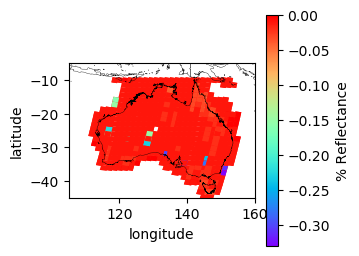
\includegraphics[scale=0.9]{plots/nbart/nbart_coastal_aerosol-MinResidual.png}
            \caption{Minimum residual}
          \end{subfigure}
%
          \begin{subfigure}[r]{.4\linewidth}
            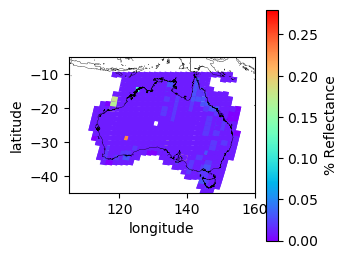
\includegraphics[scale=0.9]{plots/nbart/nbart_coastal_aerosol-MaxResidual.png}
            \caption{Maximum residual}
          \end{subfigure}
        \caption{NBART;\@ Coastal Aerosol Band}\label{figure:1}
      \end{figure}

      \begin{figure}[h!]
        \centering
          \begin{subfigure}[l]{.4\linewidth}
            \hspace{-32mm}
            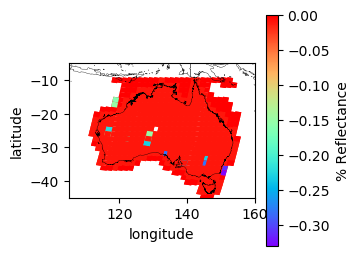
\includegraphics[scale=0.9]{plots/nbar/nbar_coastal_aerosol-MinResidual.png}
            \caption{Minimum residual}
          \end{subfigure}
%
          \begin{subfigure}[r]{.4\linewidth}
            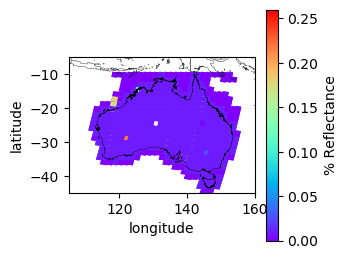
\includegraphics[scale=0.9]{plots/nbar/nbar_coastal_aerosol-MaxResidual.png}
            \caption{Maximum residual}
          \end{subfigure}
        \caption{NBAR;\@ Coastal Aerosol Band}\label{figure:2}
      \end{figure}

  \clearpage

      \begin{figure}[h!]
        \centering
          \begin{subfigure}[l]{.4\linewidth}
            \hspace{-32mm}
            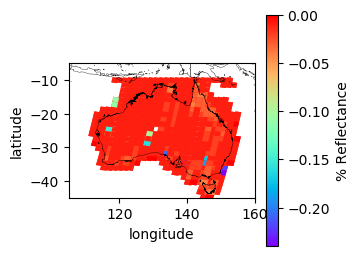
\includegraphics[scale=0.9]{plots/nbart/nbart_blue-MinResidual.png}
            \caption{Minimum residual}
          \end{subfigure}
%
          \begin{subfigure}[r]{.4\linewidth}
            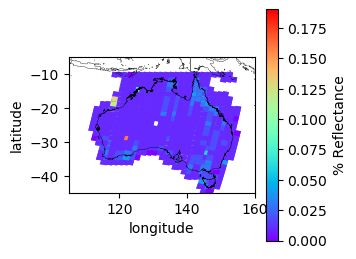
\includegraphics[scale=0.9]{plots/nbart/nbart_blue-MaxResidual.png}
            \caption{Maximum residual}
          \end{subfigure}
        \caption{NBART;\@ Blue Band}\label{figure:3}
      \end{figure}

      \begin{figure}[h!]
        \centering
          \begin{subfigure}[l]{.4\linewidth}
            \hspace{-32mm}
            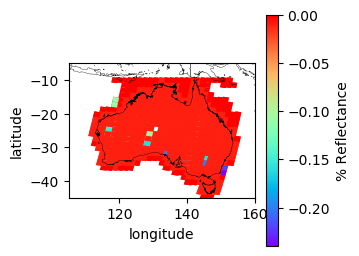
\includegraphics[scale=0.9]{plots/nbar/nbar_blue-MinResidual.png}
            \caption{Minimum residual}
          \end{subfigure}
%
          \begin{subfigure}[r]{.4\linewidth}
            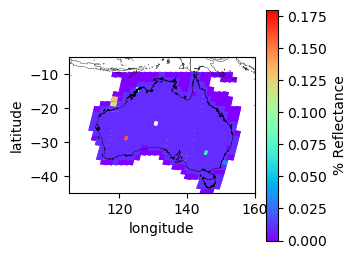
\includegraphics[scale=0.9]{plots/nbar/nbar_blue-MaxResidual.png}
            \caption{Maximum residual}
          \end{subfigure}
        \caption{NBAR;\@ Blue Band}\label{figure:4}
      \end{figure}

  \clearpage

      \begin{figure}[h!]
        \centering
          \begin{subfigure}[l]{.4\linewidth}
            \hspace{-32mm}
            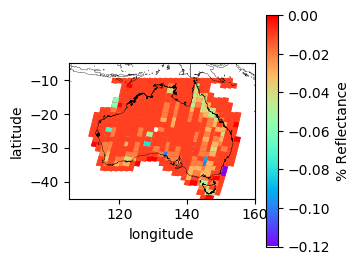
\includegraphics[scale=0.9]{plots/nbart/nbart_green-MinResidual.png}
            \caption{Minimum residual}
          \end{subfigure}
%
          \begin{subfigure}[r]{.4\linewidth}
            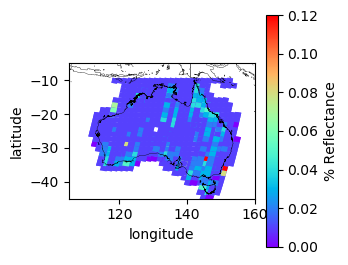
\includegraphics[scale=0.9]{plots/nbart/nbart_green-MaxResidual.png}
            \caption{Maximum residual}
          \end{subfigure}
        \caption{NBART;\@ Green Band}\label{figure:5}
      \end{figure}

      \begin{figure}[h!]
        \centering
          \begin{subfigure}[l]{.4\linewidth}
            \hspace{-32mm}
            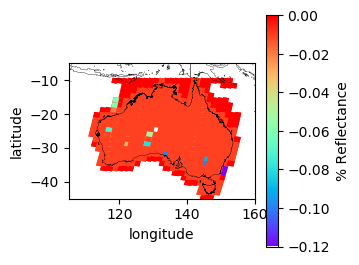
\includegraphics[scale=0.9]{plots/nbar/nbar_green-MinResidual.png}
            \caption{Minimum residual}
          \end{subfigure}
%
          \begin{subfigure}[r]{.4\linewidth}
            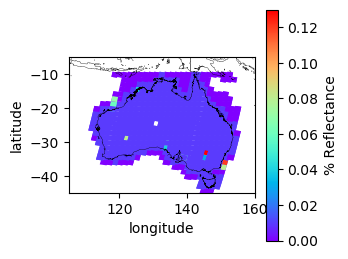
\includegraphics[scale=0.9]{plots/nbar/nbar_green-MaxResidual.png}
            \caption{Maximum residual}
          \end{subfigure}
        \caption{NBAR;\@ Green Band}\label{figure:6}
      \end{figure}

  \clearpage

      \begin{figure}[h!]
        \centering
          \begin{subfigure}[l]{.4\linewidth}
            \hspace{-32mm}
            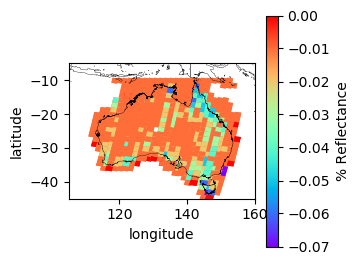
\includegraphics[scale=0.9]{plots/nbart/nbart_red-MinResidual.png}
            \caption{Minimum residual}
          \end{subfigure}
%
          \begin{subfigure}[r]{.4\linewidth}
            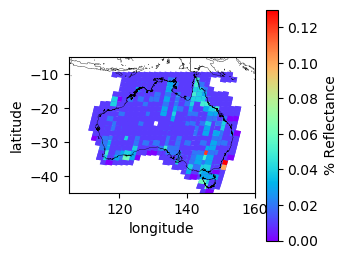
\includegraphics[scale=0.9]{plots/nbart/nbart_red-MaxResidual.png}
            \caption{Maximum residual}
          \end{subfigure}
        \caption{NBART;\@ Red Band}\label{figure:7}
      \end{figure}

      \begin{figure}[h!]
        \centering
          \begin{subfigure}[l]{.4\linewidth}
            \hspace{-32mm}
            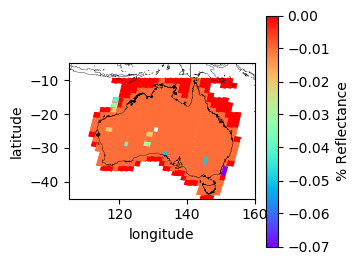
\includegraphics[scale=0.9]{plots/nbar/nbar_red-MinResidual.png}
            \caption{Minimum residual}
          \end{subfigure}
%
          \begin{subfigure}[r]{.4\linewidth}
            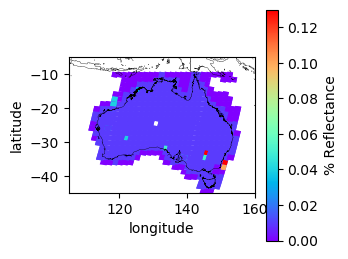
\includegraphics[scale=0.9]{plots/nbar/nbar_red-MaxResidual.png}
            \caption{Maximum residual}
          \end{subfigure}
        \caption{NBAR;\@ Red Band}\label{figure:8}
      \end{figure}

  \clearpage

      \begin{figure}[h!]
        \centering
          \begin{subfigure}[l]{.4\linewidth}
            \hspace{-32mm}
            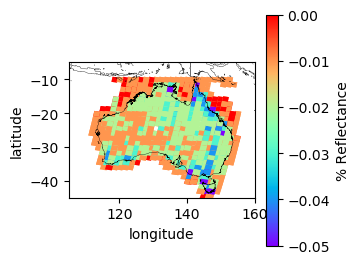
\includegraphics[scale=0.9]{plots/nbart/nbart_nir-MinResidual.png}
            \caption{Minimum residual}
          \end{subfigure}
%
          \begin{subfigure}[r]{.4\linewidth}
            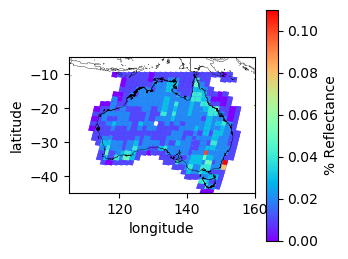
\includegraphics[scale=0.9]{plots/nbart/nbart_nir-MaxResidual.png}
            \caption{Maximum residual}
          \end{subfigure}
        \caption{NBART;\@ NIR Band}\label{figure:9}
      \end{figure}

      \begin{figure}[h!]
        \centering
          \begin{subfigure}[l]{.4\linewidth}
            \hspace{-32mm}
            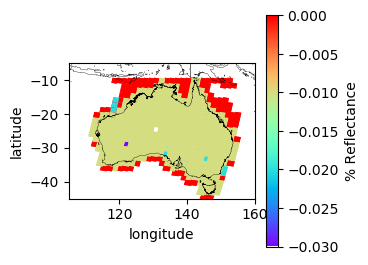
\includegraphics[scale=0.9]{plots/nbar/nbar_nir-MinResidual.png}
            \caption{Minimum residual}
          \end{subfigure}
%
          \begin{subfigure}[r]{.4\linewidth}
            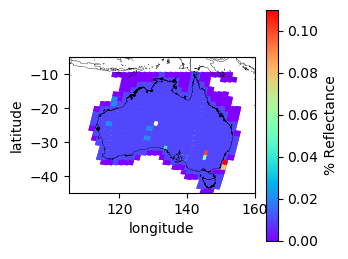
\includegraphics[scale=0.9]{plots/nbar/nbar_nir-MaxResidual.png}
            \caption{Maximum residual}
          \end{subfigure}
        \caption{NBAR;\@ NIR Band}\label{figure:10}
      \end{figure}

  \clearpage

      \begin{figure}[h!]
        \centering
          \begin{subfigure}[l]{.4\linewidth}
            \hspace{-32mm}
            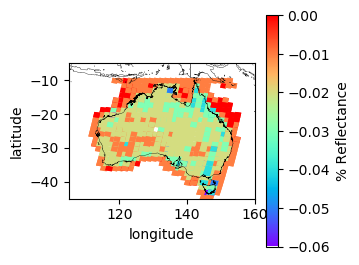
\includegraphics[scale=0.9]{plots/nbart/nbart_swir_1-MinResidual.png}
            \caption{Minimum residual}
          \end{subfigure}
%
          \begin{subfigure}[r]{.4\linewidth}
            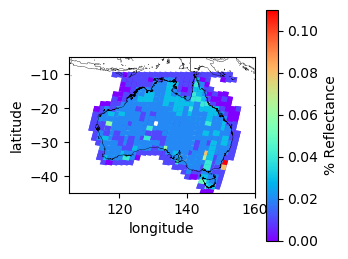
\includegraphics[scale=0.9]{plots/nbart/nbart_swir_1-MaxResidual.png}
            \caption{Maximum residual}
          \end{subfigure}
        \caption{NBART;\@ SWIR-1 Band}\label{figure:11}
      \end{figure}

      \begin{figure}[h!]
        \centering
          \begin{subfigure}[l]{.4\linewidth}
            \hspace{-32mm}
            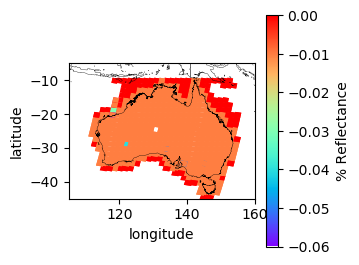
\includegraphics[scale=0.9]{plots/nbar/nbar_swir_1-MinResidual.png}
            \caption{Minimum residual}
          \end{subfigure}
%
          \begin{subfigure}[r]{.4\linewidth}
            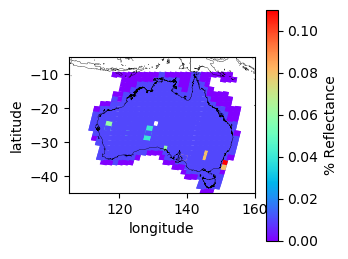
\includegraphics[scale=0.9]{plots/nbar/nbar_swir_1-MaxResidual.png}
            \caption{Maximum residual}
          \end{subfigure}
        \caption{NBAR;\@ SWIR-1 Band}\label{figure:12}
      \end{figure}

  \clearpage

      \begin{figure}[h!]
        \centering
          \begin{subfigure}[l]{.4\linewidth}
            \hspace{-32mm}
            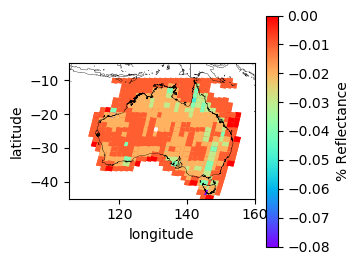
\includegraphics[scale=0.9]{plots/nbart/nbart_swir_2-MinResidual.png}
            \caption{Minimum residual}
          \end{subfigure}
%
          \begin{subfigure}[r]{.4\linewidth}
            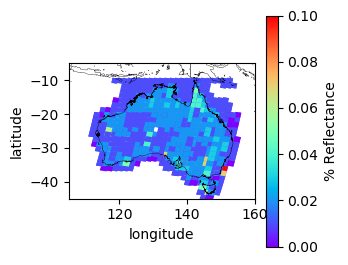
\includegraphics[scale=0.9]{plots/nbart/nbart_swir_2-MaxResidual.png}
            \caption{Maximum residual}
          \end{subfigure}
        \caption{NBART;\@ SWIR-2 Band}\label{figure:13}
      \end{figure}

      \begin{figure}[h!]
        \centering
          \begin{subfigure}[l]{.4\linewidth}
            \hspace{-32mm}
            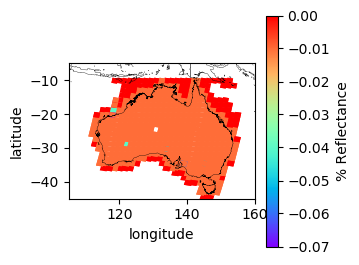
\includegraphics[scale=0.9]{plots/nbar/nbar_swir_2-MinResidual.png}
            \caption{Minimum residual}
          \end{subfigure}
%
          \begin{subfigure}[r]{.4\linewidth}
            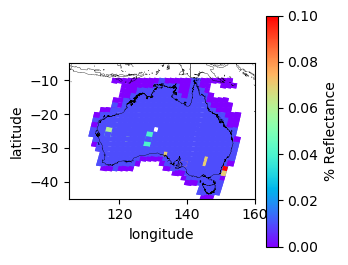
\includegraphics[scale=0.9]{plots/nbar/nbar_swir_2-MaxResidual.png}
            \caption{Maximum residual}
          \end{subfigure}
        \caption{NBAR;\@ SWIR-2 Band}\label{figure:14}
      \end{figure}

  \clearpage

      \begin{figure}[h!]
        \centering
          \begin{subfigure}[l]{.4\linewidth}
            \hspace{-32mm}
            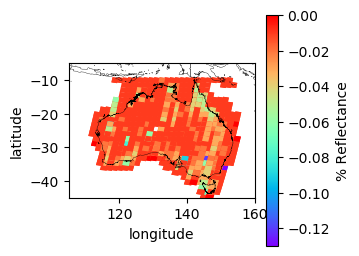
\includegraphics[scale=0.9]{plots/nbart/nbart_panchromatic-MinResidual.png}
            \caption{Minimum residual}
          \end{subfigure}
%
          \begin{subfigure}[r]{.4\linewidth}
            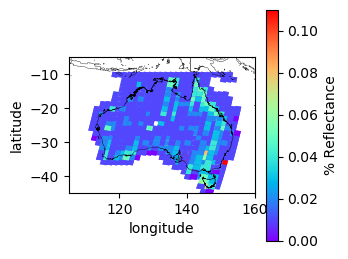
\includegraphics[scale=0.9]{plots/nbart/nbart_panchromatic-MaxResidual.png}
            \caption{Maximum residual}
          \end{subfigure}
        \caption{NBART;\@ Panchromatic Band}\label{figure:13}
      \end{figure}

      \begin{figure}[h!]
        \centering
          \begin{subfigure}[l]{.4\linewidth}
            \hspace{-32mm}
            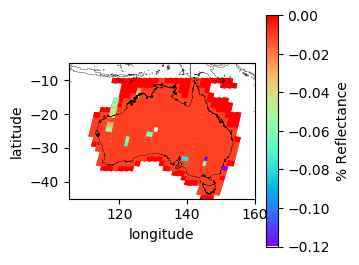
\includegraphics[scale=0.9]{plots/nbar/nbar_panchromatic-MinResidual.png}
            \caption{Minimum residual}
          \end{subfigure}
%
          \begin{subfigure}[r]{.4\linewidth}
            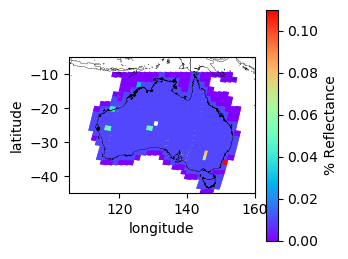
\includegraphics[scale=0.9]{plots/nbar/nbar_panchromatic-MaxResidual.png}
            \caption{Maximum residual}
          \end{subfigure}
        \caption{NBAR;\@ Panchromatic Band}\label{figure:14}
      \end{figure}

  \clearpage

    \subsubsection{Proportion of Differences (\textit{\% of pixels != 0})}

      \begin{flushleft}
        The section is to inform the spatial distribution of the proportionality of pixels that are different, i.e. the residual is != 0. \par
        Two key pieces of information can be inferred here:
        \begin{enumerate}
          \item The extremities for the proportion of non-zero residuals
          \item A spatial representation of non-zero residuals
        \end{enumerate}
      \end{flushleft}

      \begin{figure}[h!]
        \centering
          \begin{subfigure}[l]{.4\linewidth}
            \hspace{-32mm}
            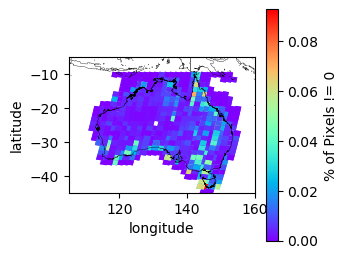
\includegraphics[scale=0.9]{plots/nbart/nbart_coastal_aerosol-PercentDifferent.png}
            \caption{NBART}
          \end{subfigure}
%
          \begin{subfigure}[r]{.4\linewidth}
            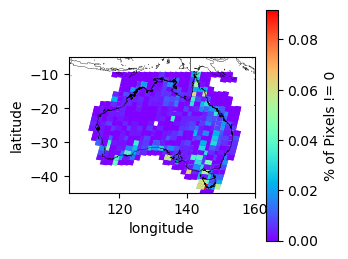
\includegraphics[scale=0.9]{plots/nbar/nbar_coastal_aerosol-PercentDifferent.png}
            \caption{NBAR}
          \end{subfigure}
        \caption{Coastal Aerosol Band \% Pixels != 0}\label{figure:15}
      \end{figure}

      \begin{figure}[h!]
        \centering
          \begin{subfigure}[l]{.4\linewidth}
            \hspace{-32mm}
            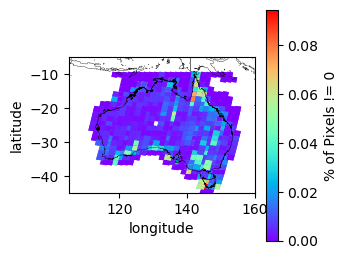
\includegraphics[scale=0.9]{plots/nbart/nbart_blue-PercentDifferent.png}
            \caption{NBART}
          \end{subfigure}
%
          \begin{subfigure}[r]{.4\linewidth}
            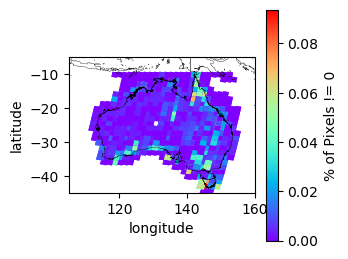
\includegraphics[scale=0.9]{plots/nbar/nbar_blue-PercentDifferent.png}
            \caption{NBAR}
          \end{subfigure}
        \caption{Blue Band \% Pixels != 0}\label{figure:16}
      \end{figure}

  \clearpage

      \begin{figure}[h!]
        \centering
          \begin{subfigure}[l]{.4\linewidth}
            \hspace{-32mm}
            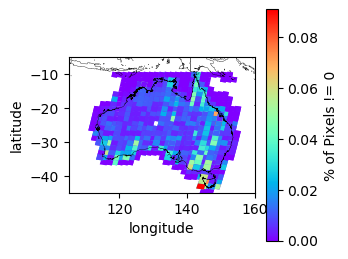
\includegraphics[scale=0.9]{plots/nbart/nbart_green-PercentDifferent.png}
            \caption{NBART}
          \end{subfigure}
%
          \begin{subfigure}[r]{.4\linewidth}
            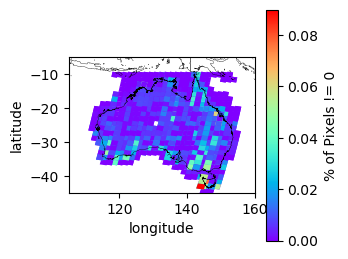
\includegraphics[scale=0.9]{plots/nbar/nbar_green-PercentDifferent.png}
            \caption{NBAR}
          \end{subfigure}
        \caption{Green Band \% Pixels != 0}\label{figure:17}
      \end{figure}

      \begin{figure}[h!]
        \centering
          \begin{subfigure}[l]{.4\linewidth}
            \hspace{-32mm}
            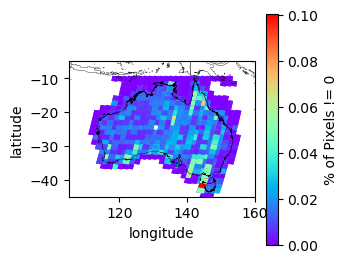
\includegraphics[scale=0.9]{plots/nbart/nbart_red-PercentDifferent.png}
            \caption{NBART}
          \end{subfigure}
%
          \begin{subfigure}[r]{.4\linewidth}
            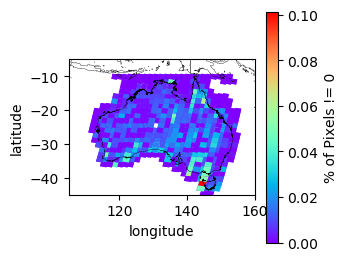
\includegraphics[scale=0.9]{plots/nbar/nbar_red-PercentDifferent.png}
            \caption{NBAR}
          \end{subfigure}
        \caption{Red Band \% Pixels != 0}\label{figure:18}
      \end{figure}

  \clearpage

      \begin{figure}[h!]
        \centering
          \begin{subfigure}[l]{.4\linewidth}
            \hspace{-32mm}
            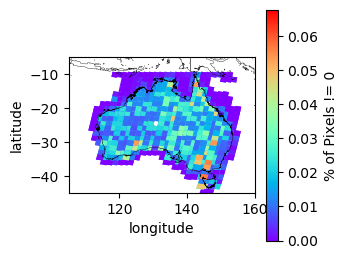
\includegraphics[scale=0.9]{plots/nbart/nbart_nir-PercentDifferent.png}
            \caption{NBART}
          \end{subfigure}
%
          \begin{subfigure}[r]{.4\linewidth}
            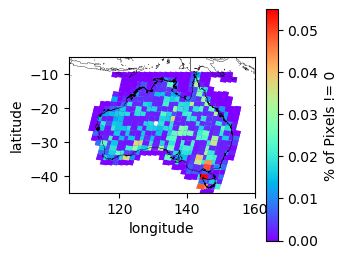
\includegraphics[scale=0.9]{plots/nbar/nbar_nir-PercentDifferent.png}
            \caption{NBAR}
          \end{subfigure}
        \caption{NIR Band \% Pixels != 0}\label{figure:19}
      \end{figure}

      \begin{figure}[h!]
        \centering
          \begin{subfigure}[l]{.4\linewidth}
            \hspace{-32mm}
            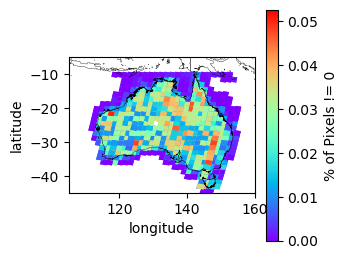
\includegraphics[scale=0.9]{plots/nbart/nbart_swir_1-PercentDifferent.png}
            \caption{NBART}
          \end{subfigure}
%
          \begin{subfigure}[r]{.4\linewidth}
            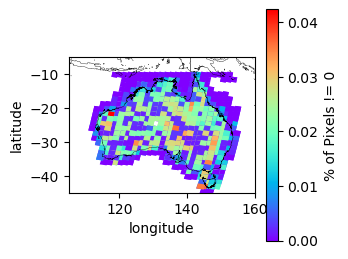
\includegraphics[scale=0.9]{plots/nbar/nbar_swir_1-PercentDifferent.png}
            \caption{NBAR}
          \end{subfigure}
        \caption{SWIR-1 Band \% Pixels != 0}\label{figure:20}
      \end{figure}

  \clearpage

      \begin{figure}[h!]
        \centering
          \begin{subfigure}[l]{.4\linewidth}
            \hspace{-32mm}
            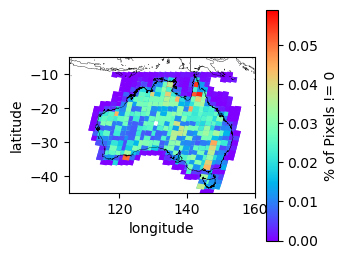
\includegraphics[scale=0.9]{plots/nbart/nbart_swir_2-PercentDifferent.png}
            \caption{NBART}
          \end{subfigure}
%
          \begin{subfigure}[r]{.4\linewidth}
            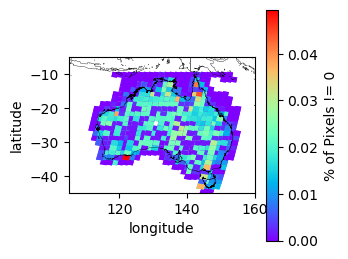
\includegraphics[scale=0.9]{plots/nbar/nbar_swir_2-PercentDifferent.png}
            \caption{NBAR}
          \end{subfigure}
        \caption{SWIR-2 Band \% Pixels != 0}\label{figure:21}
      \end{figure}

      \begin{figure}[h!]
        \centering
          \begin{subfigure}[l]{.4\linewidth}
            \hspace{-32mm}
            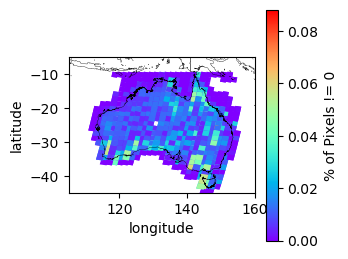
\includegraphics[scale=0.9]{plots/nbart/nbart_panchromatic-PercentDifferent.png}
            \caption{NBART}
          \end{subfigure}
%
          \begin{subfigure}[r]{.4\linewidth}
            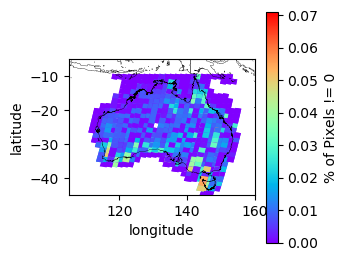
\includegraphics[scale=0.9]{plots/nbar/nbar_panchromatic-PercentDifferent.png}
            \caption{NBAR}
          \end{subfigure}
        \caption{Panchromatic Band \% Pixels != 0}\label{figure:22}
      \end{figure}

  \clearpage

  \section{Other Assessments}

    \subsection{GQA}

      \begin{flushleft}
        The calculated QGA metrics for the months worth of data, approx. 1000 granules, are consistent with those reported by the previous version deployed for the Raijin compute cluster. \par
        There were 8 granules that reported a difference in the GQA results, and the extrema are summarised in Table~\ref{table:13}, below.
      \end{flushleft}

      \begin{table}[ht!]
        \caption{Extrema \textit{(min, max)} for each GQA field; units are in pixels}\label{table:13}
        \centering
        \begin{tabular}{ccc} \midrule
          \textbf{Field} & \textbf{Minimum Difference} & \textbf{Maximum Difference} \\ \midrule
          abs\_iterative\_mean\_x & 0.02 & 0.02 \\
          abs\_iterative\_mean\_xy & 0.01 & 0.03 \\
          abs\_iterative\_mean\_y & 0.01 & 0.01 \\
          abs\_x & 0.01 & 0.01 \\
          abs\_xy & 0.01 & 0.01 \\
          abs\_y & -0.01 & 0.01 \\
          cep90 & 0.03 & 0.03 \\
          iterative\_mean\_x & -0.02 & -0.02 \\
          iterative\_mean\_xy & 0.02 & 0.02 \\
          iterative\_mean\_y & 0.01 & 0.01 \\
          iterative\_stddev\_x & 0.04 & 0.04 \\
          iterative\_stddev\_xy & 0.01 & 0.05 \\
          iterative\_stddev\_y & 0.02 & 0.02 \\
          mean\_x & 0.01 & 0.01 \\
          mean\_xy & -0.01 & -0.01 \\
          stddev\_x & -0.03 & 0.02 \\
          stddev\_xy & -0.04 & 0.04 \\
          stddev\_y & -0.04 & 0.04 \\ \midrule
        \end{tabular}
      \end{table}

      \begin{flushleft}
        Whilst there are differences, the extrema are considered to be relatively small, as well as the fact that there are only 8 of the 954 granules that are reporting a measurable change in value. \par
        We have also found differences in the GQA metrics that are immeasurable. Essentially the test data, produced from the new Gadi build, recorded usable GQA metrics, whereas the reference data records NaN's. Looking into the captured provenance file, \textit{*.proc-info.yaml}, it was recorded that \textbf{Gverify} timed out, resulting in no useable GQA metrics. \par
        Of the 954 granules, only 3 granules reported the \textit{Gverify timed out} issue, or $<$ 0.4\% of the total sample set. While it is not ideal to have such a very different mismatch, in this instance, have a usable GQA metric is better than nothing.
      \end{flushleft}

    \subsection{Software Versions}

      \begin{flushleft}
        The software versions listed in the test metadata documents \textit{*.odc-metadata.yaml}, are consistent and correct for test build used to output the sample products. \par
        The version of eodatasets3 will be bumped to 0.8.0 for the production build, and tesp version 0.6.2 will be added to the software versions list.
      \end{flushleft}

      \begin{lstlisting}
        software_versions:
        - name: modtran
          url: http://www.ontar.com/software/productdetails.aspx?item=modtran
          version: 6.0.1
        - name: wagl
          url: https://github.com/GeoscienceAustralia/wagl.git
          version: 5.4.1
        - name: eugl
          url: https://github.com/OpenDataCubePipelines/eugl.git
          version: 0.2.1
        - name: gverify
          url:
          version: v0.25c
        - name: fmask
          url: https://bitbucket.org/chchrsc/python-fmask
          version 0.5.4
        - name: eodatasets3
          url: https://github.com/GeoscienceAustralia/eo-datasets
          version: 0.6.0
      \end{lstlisting}

    \subsection{File Naming Consistency}

      \begin{flushleft}
        The output filenames for the sample set are consistent with those from the reference set.
      \end{flushleft}

    \subsection{Quicklook Images}

      \begin{flushleft}
        The quicklook images are displaying the correct band colour combinations, and the contrast stretch is consistent and not too washed out in the handful of granules selected for manual inspection.
      \end{flushleft}

  \clearpage

  \section{Conclusions}

    \begin{flushleft}
      The sample datasets for the surface reflectance measurements produced on the Gadi compute cluster are not exhibiting an extreme difference from the same set of data produced on the Raijin compute cluster. \par
      For DEA's current set of applications, a change in surface reflectance of less than 1\% should not have a significant impact on applications derived from this baseline. However, it is still recommended that any application derived from this baseline, be tested and reported on. This will aid in building a greater understanding of what is and what isn't impacted by changes in baseline data. It will also assist the ARD team in building a pipeline specifically for testing the impact on derived applications. \par
      The spatial distribution of the difference extrema, and difference proportionality, aren't exhibiting any major trends, however, there is a noticeable correlation with known surface characteristics such as hills, valleys and the North Queensland coastline. \par
      This is more noticeable for the \textit{NBART} measurements, and most likely due to the floating point differences that can occur in convolution. For your information, the \textit{NBART} workflow applies convolution to smooth the National DSM in order to reduce the amount of noise the DSM contains. \par
    \end{flushleft}

    \begin{flushleft}
      The sample datasets for the floating point \textit{object attribute} measurements do exhibit some level of change. Unfortunately, these measurements are still being thoroughly tested in order to try and define what \textbf{significant change} actually is. \par
      Currently, these measurements are mostly used for pixel level metadata, and we are defining significant change to be how much of an impact these measurements have on the surface reflectance products, \textit{NBAR} and \textit{NBART}. \par
      As we aren't reporting a significant change/impact for the surface reflectance measurements, we have agreed that whatever differences have occurred for the floating point \textit{object attributes} measurements are not significant and therefore tolerable. \par
      The sample datasets for the categorical \textit{object attribute} measurements \textit{oa\_combined\_terrain\_shadow} and \textit{oa\_nbart\_contiguity} are not exhibiting an extreme difference in change of categorical state, in either the \textit{min} or \textit{max} extrema, nor in the frequency distribution of granules that have recorded a change of categorical state. \par
      These changes are only occurring for measurements related to NBART, which suggests slight differences in the detection of shaded and unshaded terrain. \par
      We can put this down to differences in floating point operations that can occur during convolution. The ARD team see this is unavoidable, and agree that such changes are within tolerable limits, when operating in a continental context. \par
    \end{flushleft}

    \begin{flushleft}
      We do ask that users relying on this data to undertake their own comparison, if there are \textbf{significant} impacts that are derived \textbf{directly} from a change in categorical value, to notify the ARD team so we can investigate the issue further, and potentially roll out a new collection.\par
      The sample datasets for the \textit{oa\_fmask} measurement have not recorded any categorical change, ensuring complete consistency between the Raijin and Gadi environment builds.
    \end{flushleft}

    \begin{flushleft}
      The \textit{gverify timed out} issue is not new, but not something resolvable without repeatedly re-running \textbf{Gverify} and still no guarantee of success. However, in an operational context, this is an undesired. As such, a decision was made to simply record the issue as provenance, to inform the user that Gverify was not actually executed, and in time, the granule may be submitted for reprocessing.
    \end{flushleft}

  \section{Recommendations}

    \begin{flushleft}
      For the ARD Landsat Collection 3 data, it is recommended to bump the Collection version from 3.0.0 to 3.0.1. \par
      A submission to DEA's Change Control Board (CCB) regarding the recommendation will be prepared, before rolling out the new production pipeline. Updates to DEA's metadata and packaging software, eodatasets \url{https://www.github.com/GeoscienceAustralia/eo-datasets}, will be required to reflect the change in the Collection version number. \par
      It is still recommended that individual users and groups undertake an impact analysis of their own products. This report is only assessing the level of change within the ARD products, and does not attempt to assess a flow-on effect on downstream/derived products. \par
      An official production build of the specific versions listed in section~\ref{sec:environ}, along with a new release for eodatasets3, will be prepared and production restarted ASAP.
    \end{flushleft}

    \begin{flushleft}
      In regards to the \textit{gverify timed out} issue, the ARD team recommends a identifying all such records and re-running them. If the re-run results in usable GQA metrics, then the old data should be archived and replaced. \par
      The records should be very easy to identify, however, if the re-run again results in a \textit{gverify timed out}, then it is recommended to ignore and not replace. The granule itself can still be usable, however, it will be filtered out when applying GQA filters within a datacube query.
    \end{flushleft}

\end{document}
